% Options for packages loaded elsewhere
\PassOptionsToPackage{unicode}{hyperref}
\PassOptionsToPackage{hyphens}{url}
\PassOptionsToPackage{dvipsnames,svgnames,x11names}{xcolor}
%
\documentclass[
  letterpaper,
  DIV=11,
  numbers=noendperiod,
  oneside]{scrartcl}

\usepackage{amsmath,amssymb}
\usepackage{lmodern}
\usepackage{iftex}
\ifPDFTeX
  \usepackage[T1]{fontenc}
  \usepackage[utf8]{inputenc}
  \usepackage{textcomp} % provide euro and other symbols
\else % if luatex or xetex
  \usepackage{unicode-math}
  \defaultfontfeatures{Scale=MatchLowercase}
  \defaultfontfeatures[\rmfamily]{Ligatures=TeX,Scale=1}
\fi
% Use upquote if available, for straight quotes in verbatim environments
\IfFileExists{upquote.sty}{\usepackage{upquote}}{}
\IfFileExists{microtype.sty}{% use microtype if available
  \usepackage[]{microtype}
  \UseMicrotypeSet[protrusion]{basicmath} % disable protrusion for tt fonts
}{}
\makeatletter
\@ifundefined{KOMAClassName}{% if non-KOMA class
  \IfFileExists{parskip.sty}{%
    \usepackage{parskip}
  }{% else
    \setlength{\parindent}{0pt}
    \setlength{\parskip}{6pt plus 2pt minus 1pt}}
}{% if KOMA class
  \KOMAoptions{parskip=half}}
\makeatother
\usepackage{xcolor}
\usepackage[left=1in,marginparwidth=2.0666666666667in,textwidth=4.1333333333333in,marginparsep=0.3in]{geometry}
\setlength{\emergencystretch}{3em} % prevent overfull lines
\setcounter{secnumdepth}{-\maxdimen} % remove section numbering
% Make \paragraph and \subparagraph free-standing
\ifx\paragraph\undefined\else
  \let\oldparagraph\paragraph
  \renewcommand{\paragraph}[1]{\oldparagraph{#1}\mbox{}}
\fi
\ifx\subparagraph\undefined\else
  \let\oldsubparagraph\subparagraph
  \renewcommand{\subparagraph}[1]{\oldsubparagraph{#1}\mbox{}}
\fi


\providecommand{\tightlist}{%
  \setlength{\itemsep}{0pt}\setlength{\parskip}{0pt}}\usepackage{longtable,booktabs,array}
\usepackage{calc} % for calculating minipage widths
% Correct order of tables after \paragraph or \subparagraph
\usepackage{etoolbox}
\makeatletter
\patchcmd\longtable{\par}{\if@noskipsec\mbox{}\fi\par}{}{}
\makeatother
% Allow footnotes in longtable head/foot
\IfFileExists{footnotehyper.sty}{\usepackage{footnotehyper}}{\usepackage{footnote}}
\makesavenoteenv{longtable}
\usepackage{graphicx}
\makeatletter
\def\maxwidth{\ifdim\Gin@nat@width>\linewidth\linewidth\else\Gin@nat@width\fi}
\def\maxheight{\ifdim\Gin@nat@height>\textheight\textheight\else\Gin@nat@height\fi}
\makeatother
% Scale images if necessary, so that they will not overflow the page
% margins by default, and it is still possible to overwrite the defaults
% using explicit options in \includegraphics[width, height, ...]{}
\setkeys{Gin}{width=\maxwidth,height=\maxheight,keepaspectratio}
% Set default figure placement to htbp
\makeatletter
\def\fps@figure{htbp}
\makeatother

\KOMAoption{captions}{tableheading}
\makeatletter
\makeatother
\makeatletter
\makeatother
\makeatletter
\@ifpackageloaded{caption}{}{\usepackage{caption}}
\AtBeginDocument{%
\ifdefined\contentsname
  \renewcommand*\contentsname{Table of contents}
\else
  \newcommand\contentsname{Table of contents}
\fi
\ifdefined\listfigurename
  \renewcommand*\listfigurename{List of Figures}
\else
  \newcommand\listfigurename{List of Figures}
\fi
\ifdefined\listtablename
  \renewcommand*\listtablename{List of Tables}
\else
  \newcommand\listtablename{List of Tables}
\fi
\ifdefined\figurename
  \renewcommand*\figurename{Figure}
\else
  \newcommand\figurename{Figure}
\fi
\ifdefined\tablename
  \renewcommand*\tablename{Table}
\else
  \newcommand\tablename{Table}
\fi
}
\@ifpackageloaded{float}{}{\usepackage{float}}
\floatstyle{ruled}
\@ifundefined{c@chapter}{\newfloat{codelisting}{h}{lop}}{\newfloat{codelisting}{h}{lop}[chapter]}
\floatname{codelisting}{Listing}
\newcommand*\listoflistings{\listof{codelisting}{List of Listings}}
\makeatother
\makeatletter
\@ifpackageloaded{caption}{}{\usepackage{caption}}
\@ifpackageloaded{subcaption}{}{\usepackage{subcaption}}
\makeatother
\makeatletter
\@ifpackageloaded{tcolorbox}{}{\usepackage[many]{tcolorbox}}
\makeatother
\makeatletter
\@ifundefined{shadecolor}{\definecolor{shadecolor}{rgb}{.97, .97, .97}}
\makeatother
\makeatletter
\@ifpackageloaded{sidenotes}{}{\usepackage{sidenotes}}
\@ifpackageloaded{marginnote}{}{\usepackage{marginnote}}
\makeatother
\makeatletter
\makeatother
\ifLuaTeX
  \usepackage{selnolig}  % disable illegal ligatures
\fi
\IfFileExists{bookmark.sty}{\usepackage{bookmark}}{\usepackage{hyperref}}
\IfFileExists{xurl.sty}{\usepackage{xurl}}{} % add URL line breaks if available
\urlstyle{same} % disable monospaced font for URLs
\hypersetup{
  pdftitle={OpenAI's text classifier won't calm fears about AI-written homework},
  pdfauthor={Brian Tarran},
  colorlinks=true,
  linkcolor={blue},
  filecolor={Maroon},
  citecolor={Blue},
  urlcolor={Blue},
  pdfcreator={LaTeX via pandoc}}

\title{OpenAI's text classifier won't calm fears about AI-written
homework}
\author{Brian Tarran}
\date{02/16/2023}

\begin{document}
\maketitle
\ifdefined\Shaded\renewenvironment{Shaded}{\begin{tcolorbox}[boxrule=0pt, borderline west={3pt}{0pt}{shadecolor}, enhanced, frame hidden, interior hidden, sharp corners, breakable]}{\end{tcolorbox}}\fi

\renewcommand*\contentsname{Table of contents}
{
\hypersetup{linkcolor=}
\setcounter{tocdepth}{3}
\tableofcontents
}
When ChatGPT launched in December, it wasn't long before users
highlighted
\href{https://news.sky.com/story/the-ultimate-homework-cheat-how-teachers-are-facing-up-to-chatgpt-12780601}{the
tool's potential as a homework aid}. Pop an essay question into
ChatGPT's prompt box, or feed your creative writing task to the AI
instead, \emph{et voila} -- your work is done!

In reality, of course, it's not quite so simple as that. ChatGPT, like
other large language models, has an unfortunate
\href{https://realworlddatascience.net/news-and-views/editors-blog/posts/2023/01/27/talking-chatgpt.html}{habit
of making stuff up} -- fine for creative writing, perhaps; not so good
for a history essay. Outputs need to be checked and verified if you want
to guarantee a good mark on your assignments. But while ChatGPT can't --
and shouldn't -- be trusted completely, many have found that it can help
lighten the homework load.

With
\href{https://www.theguardian.com/technology/2023/feb/02/chatgpt-100-million-users-open-ai-fastest-growing-app}{ChatGPT's
user count crossing the 100 million mark} this month, it's
understandable that worries about an explosion of AI-written text have
proliferated the education profession.
\href{https://www.washingtonpost.com/education/2023/01/05/nyc-schools-ban-chatgpt/}{Some
education systems} have decided to
\href{https://www.smh.com.au/national/nsw/can-you-tell-between-a-year-6-student-and-ai-teachers-say-they-can-20230120-p5ce5s.html}{ban
the use of ChatGPT}. Other educators have adopted a more relaxed
approach. Writing in \emph{Scientific American},
\href{https://www.scientificamerican.com/article/how-chatgpt-can-improve-education-not-threaten-it/}{law
professor John Villasenor argued}:

\begin{quote}
``The time when a person had to be a good writer to produce good writing
ended in late 2022, and we need to adapt. Rather than banning students
from using labor-saving and time-saving AI writing tools, we should
teach students to use them ethically and productively\ldots{} They need
to learn to compose well-organized, coherent essays involving a mix of
AI-generated text and traditional writing.''
\end{quote}

Villasenor makes a valid point. But experience tells us that not every
student is going to use these tools ethically. Some will pursue the path
of least resistence and will attempt to pass off ChatGPT's outputs as
their own. So, the question becomes: Is it possible to tell the
difference between human-generated text and AI-generated text?

One answer to that question comes from OpenAI, makers of ChatGPT. On
January 31, they launched a classifier ``to distinguish between text
written by a human and text written by AIs from a variety of
providers''.

OpenAI introduces the classifier by saying that reliably detecting
\emph{all} AI-written text is ``impossible''. But it goes on to say:

\begin{quote}
``\ldots{} we believe good classifiers can inform mitigations for false
claims that AI-generated text was written by a human: for example,
running automated misinformation campaigns, using AI tools for academic
dishonesty, and positioning an AI chatbot as a human.''
\end{quote}

OpenAI stresses that the current version of the classifier ``should not
be used as a primary decision-making tool'', and users should take that
statement to heart -- especially if they are planning to vet student
homework with it. In evaluations, OpenAI reports that its classifer
\textbf{correctly identifies AI-written text as ``likely AI-written''
only 26\% of the time}, while \textbf{human written text is incorrectly
labelled as AI-written 9\% of the time}.

These two reported numbers are important, but they don't directly answer
the question that most educators will be asking. ``If a piece of
homework is flagged as `likely AI-written', what is the probability that
it actually is?''

A version of this question will be familiar to medical statisticians,
who often find themselves having to explain screening test outcomes --
specifically, the probability that a person has disease X given that
they have tested positive for the disease. This probability depends on
both the \textbf{prevalence} of a disease and the \textbf{sensitivity}
and \textbf{specificity} of the test.

Writing for
\href{https://www.significancemagazine.com/science/547-a-visual-guide-to-screening-test-results?highlight=WyJzY3JlZW5pbmciXQ==}{significancemagazine.com}
in 2017, Tim Brock gave a nice explainer of these terms:

\begin{itemize}
\item
  \begin{description}
  \tightlist
  \item[Prevalence]
  The proportion of the population being tested that are affected by a
  given condition.
  \end{description}
\item
  \begin{description}
  \tightlist
  \item[Sensitivity]
  The proportion of patients with the condition being screened for that
  are correctly identified as having the condition.
  \end{description}
\item
  \begin{description}
  \tightlist
  \item[Specificity]
  The proportion of patients without the condition being screened for
  that are correctly identified as not having the condition.
  \end{description}
\end{itemize}

We know from OpenAI's own evaluations that out of 100 pieces of
AI-written text, only 26 would be classified as ``likely AI-written'',
so the classifier's sensitivity is 26\%. And out of 100 pieces of
human-written text, 9 would be classified as AI written, so specificity
is (100--9) = 91\%. But the big piece of information we don't know is
prevalence: What proportion of homework assignments are written by AI?

Let's be conservative for a moment and assume that 5\% of homework
assignments are AI-generated. If you were screening 1,000 pieces of
homework with the OpenAI classifier, you'd see the following results:

\begin{longtable}[]{@{}
  >{\raggedright\arraybackslash}p{(\columnwidth - 8\tabcolsep) * \real{0.1200}}
  >{\raggedleft\arraybackslash}p{(\columnwidth - 8\tabcolsep) * \real{0.2133}}
  >{\raggedleft\arraybackslash}p{(\columnwidth - 8\tabcolsep) * \real{0.2267}}
  >{\raggedleft\arraybackslash}p{(\columnwidth - 8\tabcolsep) * \real{0.2133}}
  >{\raggedleft\arraybackslash}p{(\columnwidth - 8\tabcolsep) * \real{0.2267}}@{}}
\toprule()
\begin{minipage}[b]{\linewidth}\raggedright
\end{minipage} & \begin{minipage}[b]{\linewidth}\raggedleft
True positives
\end{minipage} & \begin{minipage}[b]{\linewidth}\raggedleft
False positives
\end{minipage} & \begin{minipage}[b]{\linewidth}\raggedleft
True negatives
\end{minipage} & \begin{minipage}[b]{\linewidth}\raggedleft
False negatives
\end{minipage} \\
\midrule()
\endhead
Results & 13 & 86 & 864 & 37 \\
\bottomrule()
\end{longtable}

The figures below show the results graphically as proportions of (a) all
tests and (b) all positive tests.

\begin{figure}

{\centering 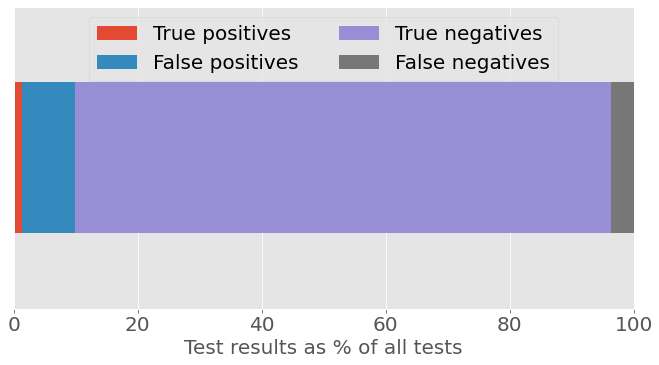
\includegraphics{fig1a.png}

}

\end{figure}

\marginnote{\begin{footnotesize}

\textbf{Figure 1a:} Classifier test results as a percentage of all
tests, assuming 5\% prevalence of AI-written homework.

\end{footnotesize}}

\begin{figure}

{\centering 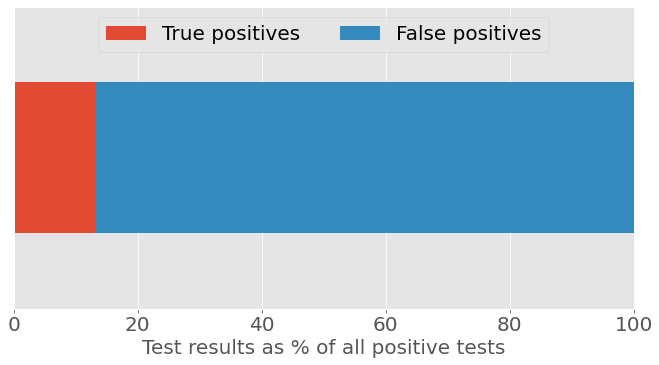
\includegraphics{fig1b.png}

}

\end{figure}

\marginnote{\begin{footnotesize}

\textbf{Figure 1b:} Classifier test results as a percentage of all
positive tests, assuming 5\% prevalence of AI-written homework.

\end{footnotesize}}

From Figure 1b specifically, we can see that if the classifier delivers
a ``likely AI-written'' result, the chance that the text is AI-written
is only about 13\%. This is the classifier's
\href{https://uk.cochrane.org/news/sensitivity-and-specificity-explained-cochrane-uk-trainees-blog}{positive
predictive value} in this scenario.

Of course, the prevalence of AI-written homework is likely to vary based
on where students live, what age they are, their level of interest in AI
tools and technologies, and many other factors.
\href{https://stanforddaily.com/2023/01/22/scores-of-stanford-students-used-chatgpt-on-final-exams-survey-suggests/}{A
poll of Stanford University students by The Stanford Daily}, for
example, found that 17\% of respondents used ChatGPT for final
assignments or exams in the fall quarter -- though it reports that
``only about 5\% reported having submitted written material directly
from ChatGPT with little to no edits''.

But if we reproduce our figures using a prevalence rate of 17\%, the
chance that a positive result is a true positive is now about 37\%.

\begin{longtable}[]{@{}
  >{\raggedright\arraybackslash}p{(\columnwidth - 8\tabcolsep) * \real{0.1200}}
  >{\raggedleft\arraybackslash}p{(\columnwidth - 8\tabcolsep) * \real{0.2133}}
  >{\raggedleft\arraybackslash}p{(\columnwidth - 8\tabcolsep) * \real{0.2267}}
  >{\raggedleft\arraybackslash}p{(\columnwidth - 8\tabcolsep) * \real{0.2133}}
  >{\raggedleft\arraybackslash}p{(\columnwidth - 8\tabcolsep) * \real{0.2267}}@{}}
\toprule()
\begin{minipage}[b]{\linewidth}\raggedright
\end{minipage} & \begin{minipage}[b]{\linewidth}\raggedleft
True positives
\end{minipage} & \begin{minipage}[b]{\linewidth}\raggedleft
False positives
\end{minipage} & \begin{minipage}[b]{\linewidth}\raggedleft
True negatives
\end{minipage} & \begin{minipage}[b]{\linewidth}\raggedleft
False negatives
\end{minipage} \\
\midrule()
\endhead
Results & 44 & 75 & 755 & 126 \\
\bottomrule()
\end{longtable}

\begin{figure}

{\centering 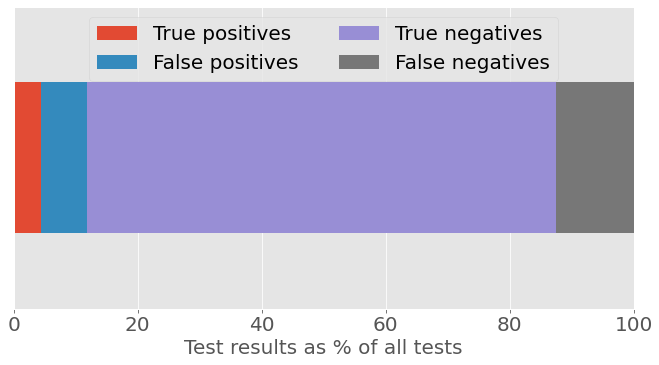
\includegraphics{fig2a.png}

}

\end{figure}

\marginnote{\begin{footnotesize}

\textbf{Figure 2a:} Classifier test results as a percentage of all
tests, assuming 17\% prevalence of AI-written homework.

\end{footnotesize}}

\begin{figure}

{\centering 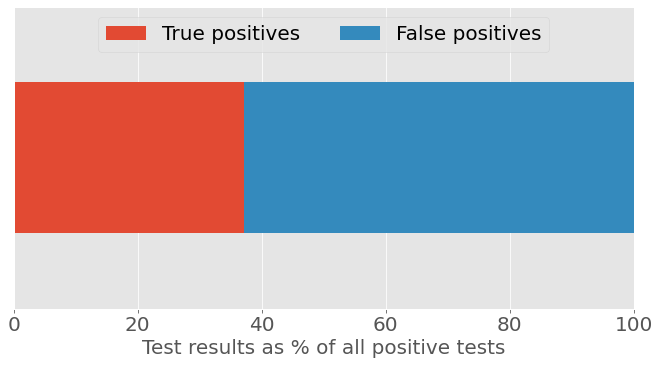
\includegraphics{fig2b.png}

}

\end{figure}

\marginnote{\begin{footnotesize}

\textbf{Figure 2b:} Classifier test results as a percentage of all
positive tests, assuming 17\% prevalence of AI-written homework.

\end{footnotesize}}

Yet another survey,
\href{https://www.prweb.com/releases/intelligent_com_survey_finds_30_percent_of_college_students_use_artificial_intelligence_chatbot_chatgpt_for_written_homework/prweb19141759.htm}{this
one from Intelligent.com}, claims that 30\% of college students have
used ChatGPT for written homework. Plugging this number into our
calculations, the chance that a positive test result is a true positive
is now slightly better than 50/50.

\begin{longtable}[]{@{}
  >{\raggedright\arraybackslash}p{(\columnwidth - 8\tabcolsep) * \real{0.1200}}
  >{\raggedleft\arraybackslash}p{(\columnwidth - 8\tabcolsep) * \real{0.2133}}
  >{\raggedleft\arraybackslash}p{(\columnwidth - 8\tabcolsep) * \real{0.2267}}
  >{\raggedleft\arraybackslash}p{(\columnwidth - 8\tabcolsep) * \real{0.2133}}
  >{\raggedleft\arraybackslash}p{(\columnwidth - 8\tabcolsep) * \real{0.2267}}@{}}
\toprule()
\begin{minipage}[b]{\linewidth}\raggedright
\end{minipage} & \begin{minipage}[b]{\linewidth}\raggedleft
True positives
\end{minipage} & \begin{minipage}[b]{\linewidth}\raggedleft
False positives
\end{minipage} & \begin{minipage}[b]{\linewidth}\raggedleft
True negatives
\end{minipage} & \begin{minipage}[b]{\linewidth}\raggedleft
False negatives
\end{minipage} \\
\midrule()
\endhead
Results & 78 & 63 & 637 & 222 \\
\bottomrule()
\end{longtable}

\begin{figure}

{\centering 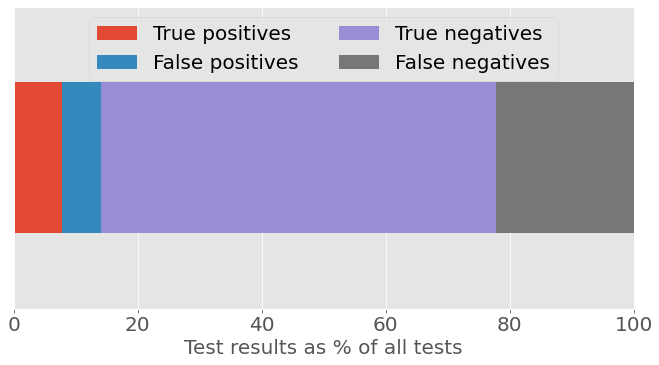
\includegraphics{fig3a.png}

}

\end{figure}

\marginnote{\begin{footnotesize}

\textbf{Figure 3a:} Classifier test results as a percentage of all
tests, assuming 30\% prevalence of AI-written homework.

\end{footnotesize}}

\begin{figure}

{\centering 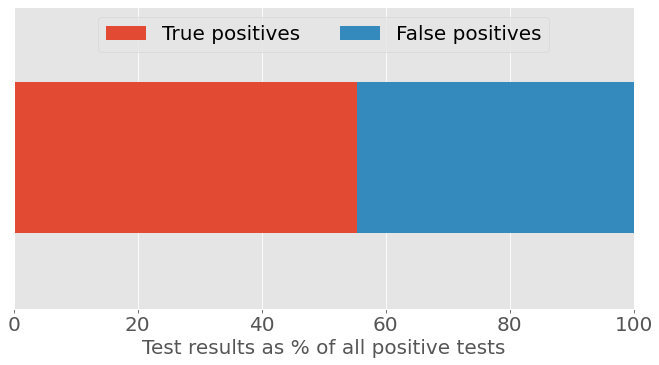
\includegraphics{fig3b.png}

}

\end{figure}

\marginnote{\begin{footnotesize}

\textbf{Figure 3b:} Classifier test results as a percentage of all
positive tests, assuming 30\% prevalence of AI-written homework.

\end{footnotesize}}

Better, sure. But 50/50 is still fairly shaky ground on which to accuse
someone of getting ChatGPT to do their homework, without any other
evidence to hand!



\end{document}
